\chapter{Estado del Arte}
\label{sec:EstadoDelArte}
La metrología de vista única está captando cada vez más atención dentro de la comunidad
científica y tecnológica debido a su enorme potencial para transformar cómo obtenemos información espacial
a partir de una sola imagen (véase la Figura~\ref{fig:ScopusSearch}). Esta técnica reduce
significativamente los costes y complejidad de los sistemas de metrología, resultando
altamente atractiva en aplicaciones móviles, industriales y de bajo presupuesto. Además,
los avances en visión por computador e inteligencia artificial permiten mejorar y ampliar
el uso y aplicabilidad de estos métodos. Profundizar en la investigación de la metrología de vista única
no solo abre nuevas fronteras tecnológicas, sino que también responde a una necesidad creciente de
soluciones más accesibles, precisas y eficientes.
\begin{figure}[htp]
\begin{center}
    \subfloat{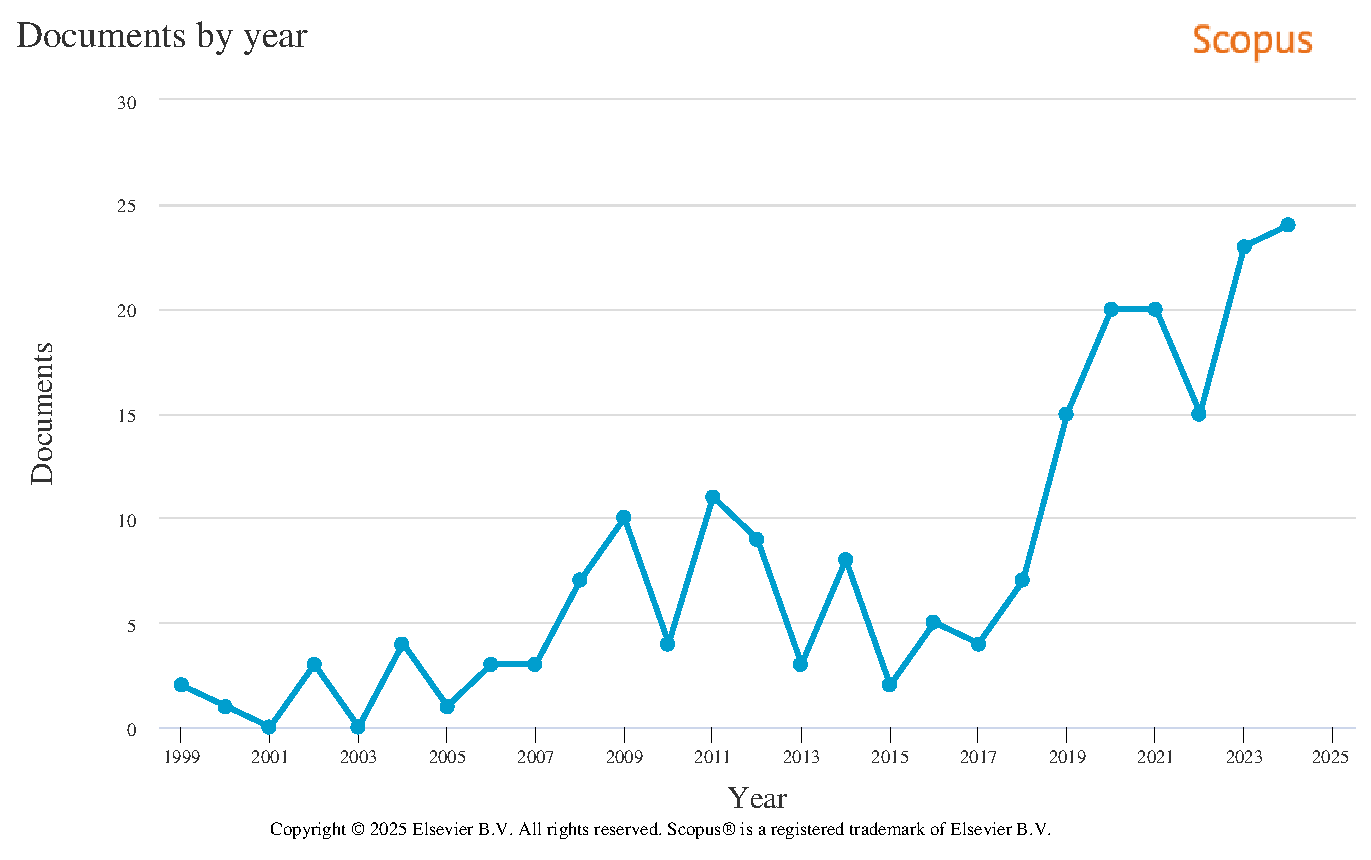
\includegraphics[width=0.5\textwidth]{imagenes/chapter3/Scopus-Analyze-Year}}
    \subfloat{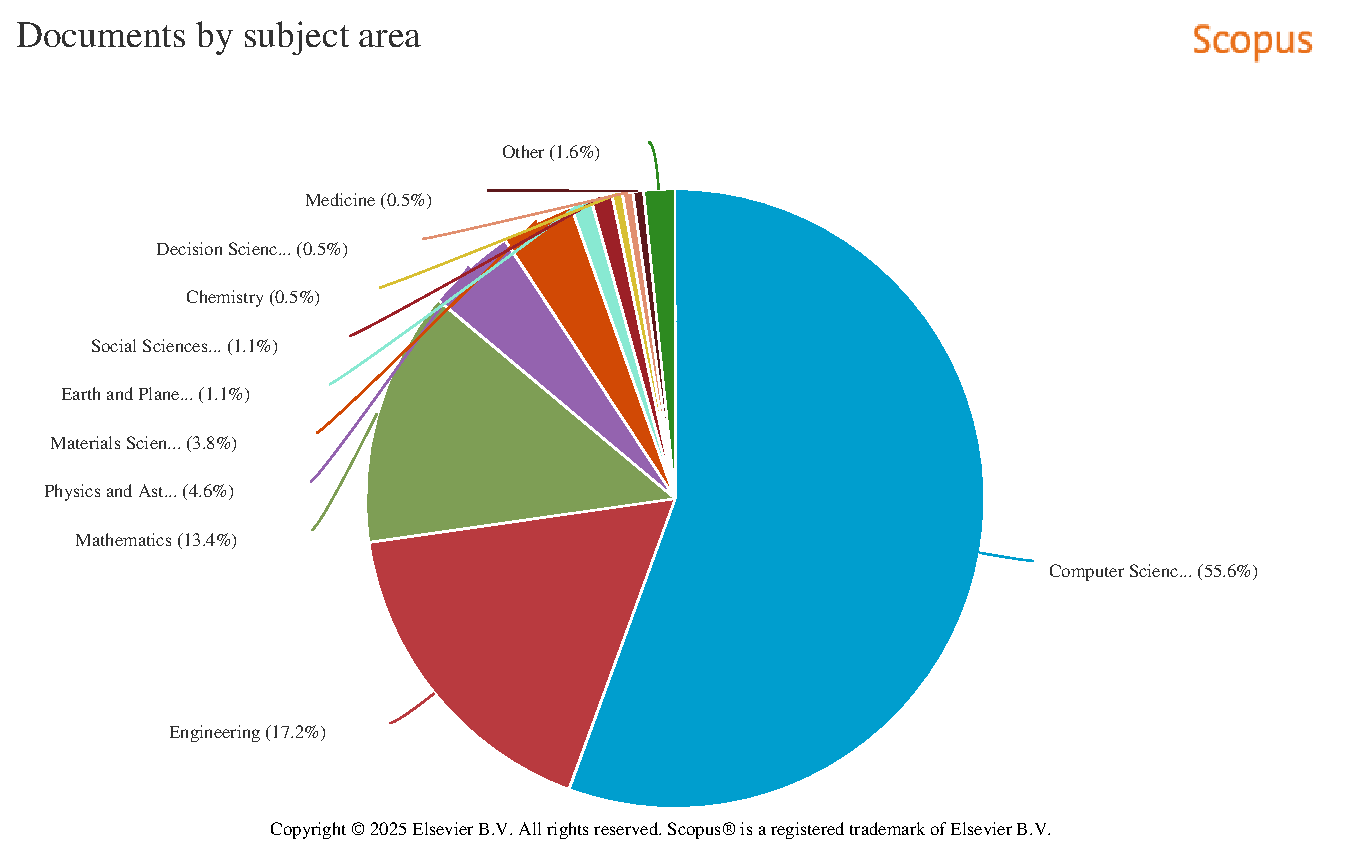
\includegraphics[width=0.5\textwidth]{imagenes/chapter3/Scopus-Analyze-Subject}}
\end{center}
\caption{Se observa, a la izquierda, una tendencia creciente en interés al campo de metrología de vista única, dado el incremento en número de publicaciones en los últimos años.
A la derecha, se describe las áreas con mayor interés, destacan la ingeniería y ciencia de la computación. }
\label{fig:ScopusSearch}
\end{figure}
\par
La metrología de vista única es un área de la visión por computador que busca extraer información métrica
tridimensional a partir de una única imagen, típicamente capturada por una cámara con proyección perspectiva.
Esta tarea implica resolver un reto significativo, dada la pérdida de información de profundidad que ocurre
durante una proyección del espacio 3D al espacio 2D. No obstante, se vuelve viable al explotar ciertas
invariantes geométricas del espacio proyectivo, como los puntos de fuga, las líneas de horizonte y las
homografías de planos.
\par
Uno de los trabajos seminales en este ámbito es el de Criminisi \emph{et al}~\cite{CriminisiReconstruction,CriminisiApplications},
que sentó las bases metodológicas para una metrología métrica a partir de una sola vista. En este trabajo,
se describen técnicas, robustas para estimar distancias, proporciones y relaciones ortogonales empleando herramientas como el
ratio cruzado, la localización de los puntos de fuga, en combinación con información de escala proveniente de objetos de referencia
en la escena.
\par
Durante los años posteriores, diversos trabajos extendieron este enfoque geométrico. Por ejemplo, Chen \emph{et al}~\cite{Chen2006}
propusieron algoritmos más robustos para imágenes no calibradas. Sin embargo, estos métodos seguían dependiendo fuertemente de
suposiciones geométricas ideales, como la presencia clara de planos ortogonales o líneas paralelas en escena. Además de necesitar
información de la escala de un objeto de referencia en la imagen, para poder extrapolar la escala absoluta de otros elementos.
\par
Con el avance de la visión por computador y el aumento en la disponibilidad de datos y poder computacional, comenzó a emerger una
transición hacia enfoques más flexibles basados en aprendizaje. Un punto de inflexión fue el trabajo de \emph{Make3D}~\cite{Make3D},
combinando principios geométricos con modelos de aprendizaje.  Este enfoque híbrido marcó el inicio de un cambio de paradigma,
los sistemas comenzaron a aprender relaciones espaciales directamente de los datos, como en el trabajo de David~\emph{et al}~\cite{DepthMapMultiScale}.
En él, se utiliza dos redes neuronales profundas, una para predecir información de profundidad global que se refina posteriormente
a trozos por la segunda.
\par
La culminación de esta transición puede observarse en el trabajo de Zhu~\emph{et al}~\cite{SVMIW}. En lugar de depender de estructuras
geométricas visibles o calibraciones manuales, este enfoque utiliza redes profundas entrenadas con objetos de referencia comunes (como humanos
y automóviles) para inferir escala y geometría en entornos reales y no estructurados. Este método representa una nueva generación
de metrología visual, donde el conocimiento geométrica está implícito en el modelo aprendido y no codificado de forma explícita.
Así, el campo ha evolucionado desde un enfoque determinista y teóricamente riguroso hacia métodos basados en aprendizaje, más adaptativos,
escalables y aplicables en condiciones del mundo real. Esta transición no solo refleja un cambio metodológico, si no también una ampliación
significativa en el alcance y accesibilidad de la metrología de vista única en aplicaciones modernas como realidad aumentada o navegación
autónoma.
